%Sample of text file to include all the documents

\documentclass[12pt,LUDisStyle,twosided]{book}
\usepackage[hang,small,bf]{caption}
\usepackage{LUDisStyle}
\usepackage{graphicx}
\usepackage{subfigure}
\usepackage{amsmath}
\usepackage{amssymb}
\usepackage{amsthm}
\usepackage{verbatim}
\usepackage{multirow}
\usepackage[square,numbers]{natbib}
\renewcommand{\topfraction}{0.95}
\renewcommand{\textfraction}{0.05}
\renewcommand{\floatpagefraction}{0.85}
\addtolength{\belowcaptionskip}{10pt}
\newcommand{\mc}{\mathcal}

\begin{document}
\pagestyle{plain}
\pagenumbering{roman}
\dissertationtrue
\thispagestyle{empty}%

	\vskip0.5in%

	\begin{center}

		\LARGE Model fidelity and its impact on power grid resource planning under high renewable penetration

	\end{center}

	\vfill

	\begin{center}

		\rm by \\
		
                         \vfill
                 
		Daniel Xavier Wolbert \\

	\end{center}

	\vfill

	\begin{center}

		\rm A Thesis \\

		Presented to the Graduate Committee \\

		of Lehigh University \\

		in Candidacy for the Degree of \\

		Master of Science \\

		in \\

		Industrial and Systems Engineering

	\end{center}

	\vfill

	\begin{center}

		Lehigh University \\

		05/2106 \\

	\end{center}\vskip.5in
	
	\newpage

%put copyright info on second page
\vspace*{\fill}
\begin{center}
Copyright\\
Daniel Xavier Wolbert
\end{center}
\newpage
%Sample signature page

\thispagestyle{plain}

Approved and recommended for acceptance as a thesis in partial fulfilment of the requirements for the degree of Master of Science.
\\
\\
Daniel Xavier Wolbert \\
Model fidelity and its impact on power grid resource planning under high renewable penetration

\vspace{.1in}

\begin{tabular}{l}
\\
\hline
\textbf{05/06/2016 \ \ \ \ \ \ \ \ \ \ \ \ \ \ \ \ \ \ \ }
\end{tabular}

\begin{flushright}
\begin{tabular}{l}
\\
\hline
\textbf{Robert H. Storer}, Thesis Director, Chair \\ 
\textbf{(Must Sign with Blue Ink)}
\end{tabular}

\vspace{.05in}

\end{flushright}

\begin{tabular}{l}
\\
\hline
\textbf{Accepted Date \ \ \ \ \ \ \ }
\end{tabular}


\begin{flushright}
\begin{tabular}{l}
Committee Members \ \ \ \ \ \ \ \ \ \ \ \ \ \ \ \ \ \ \ \ \ \ \ \ \ \
\\ 
\\
\\
\hline
\textbf{Tamas Terlaky}, Chairperson of Department\\
\\ 
\\
\\

\end{tabular}
\end{flushright}
\newpage
\chapter*{Acknowledgements}

I would like to thank the Industrial and Systems Engineering department at Lehigh University to provide me help and guidance. A special thanks to Prof. Robert H. Storer to be my supervisor and give me the necessary support to achieve my objectives.

Also, I would like to thank Dr. Dimitri Papageorgiou and his team to help me with all the data and necessary technical support, as well as professional advices.

I would like to thank the CAPES on behalf of the brazilian government to sponsor me and provide me everything necessary to achieve my goals. Finally, I would like to thank my family, my future wife and my friends in US and Brazil for their continuous moral support and positive energies. I could not express in words how grateful I am.
\tableofcontents
\nopagebreak
\addcontentsline{toc}{chapter}{List of Tables}
\listoftables
\addcontentsline{toc}{chapter}{List of Figures}
\listoffigures
\newpage
\pagestyle{plain}
\pagenumbering{arabic}
\addcontentsline{toc}{chapter}{Abstract}
\include{myabstract}
\pagestyle{plain}

\addcontentsline{toc}{chapter}{Introduction}
\chapter{Introduction}

Variable Energy Resources (usually refereed as VERs) plays an important role in the energy grid nowadays. It is expected that in 2020, x\% of all average consumed power in United States comes from them. One of important characteristics of them is the uncertain behaviour of generation pattern. With the deregulation of the energy market and the decarbonization rules, the grid operators have the challenge to plan efficiently their non-renewable resources (such as oil, coal and gas) in order to keep satisfy grid security and reliability parameters while running the grid at a minimal cost. This work analyses the classical LP version of Economic Dispatch (known as ED) and a MIP instance of Unit Commitment(UC) under different operational constraints and VERs penetration  scenarios.

\addcontentsline{toc}{chapter}{Literature Review}
\chapter{Literature Review}


The first optimal power flow formulation was proposed by <put the guy here in 1962>

\citeauthor{connolly} reviews 68 tools to power grid planning with renewable resources, discussing at the end goals, limitations and features of 37 tools \cite{connolly}. The authors emphasize that, although all the tools are essential to an accurate power planning with renewable resources, there is no perfect tool, and it should be chosen accordingly to project goals, data limitations, horizon and other features. 

\citeauthor{yamin} discusses different techniques to solve the unit commitment and economic dispatch problems, categorizing them in deterministic, heuristic or stochastic, pointing out the computational challenges and the quality of results for each one of them \cite{yamin}. 

\citeauthor{bertsimas} proposes a two-stage robust optimization to mitigate demand and variability uncertainties to solve UC when renewable resources are a major key in the field. The authors states the advantages of the method comparing to traditional reserves planning. \cite{bertsimas}

\citeauthor{padhy} formulates the unit commitment as a general optimization problem and presents a bibliographical survey of the main techniques in the last 30 years, from exhaustive methods such as priority listing, dynamic programming, mixed integer-programming  until complex heuristics like fuzzy programming, genetic algorithms and evolutionary programming, emphasizing that these one were not exhaustively tested yet. Models can be classified according to different features, that include:

\begin{enumerate}
\item Time frame: decade, year, hour, sub hour 
\item Scale: global, national, regional, local
\item Deterministic vs stochastic
\item Optimization vs Simulation
\item Algorithmic vs Heuristic
\end{enumerate}

\citeauthor{cain} categorizes the general power flow according to 3 major categories: Power Flow (PF), Economic Dispatch (ED) and Optimal Power Flow (OPF) and describe them based on the assumptions and operational constraints, as shown in table \ref{table:PowerSystemsCat} \cite{cain}.

\citeauthor{kassakian} discusses the main changes and challenges in the power system for the next years. One of important changes is the increase of VERs, that might have substantially impacts in operating costs, primarily due to the necessity of more reserve generations with different time responses \cite{kassakian}. To mitigate it, 3 suggestions were proposed: improve wind and solar forecast techniques; expand the cooperation and interconnections among regions; reduce decision horizon and resolution levels, to capture a more realistic ramping and reserve effects.

\citeauthor{palmintier} studies the impact of UC models with expansion planning, enhancing that ignoring operating constraints on an expansion planning with VERs could provide higher operating costs and fuel emissions. \cite{palmintier}. \citeauthor{hargreaves} proposes a method that combines simulation and stochastic UC to capture precisely the challenges of expanding the capacity with VERs. \cite{hargreaves}.


Under a scenario where VERs have a considerable penetration in the power system, it is necessary to study their impact. \citeauthor{deane} evaluates the UC and ED results at different solving temporal resolutions under one year. The authors discuss that sub-hourly resolutions can deal more accurately with non-thermal inflexibilities, renewable demand variabilities and ramping behaviours than one-hour resolution \cite{deane}. 

One of the alternatives studied in the literature is the use of storage devices to stock energy when the demand is lower than the capacity and use it on an abrupt peak demand, avoiding the use of conventional generators.\citeauthor{safaei} studies different storage technologies and their impact in the emission grid at a 15 minutes time resolution, without transmission constraints and forecast errors. The main insights are that cheap storage does not have major impact in the cost of reducing the carbonization, and seasonal storage are not economically justifiable. \cite{safaei}. In the other hand, \citeauthor{harris} studies the viability of seasonal storage by analysing UC results of different storage scenarios and technologies on a city level, concluding that seasonal storage can bring operational benefits and reduce operating costs and fuel emissions in peak levels.
 
\citeauthor{dwyer} investigates the effect of storage for ED and stochastic UC plannings under a sub-hourly resolution, concluding that storage can improve system stability and reduce cyclical ramping rates for NVERs, saving operation costs. 


% Please add the following required packages to your document preamble:
% \usepackage{multirow}
\begin{table}[h]
\centering
\caption{Optimal power flow categories \cite{cain}}
\label{table:PowerSystemsCat}
\begin{tabular}{|l|l|l|l|l|l|l|l|}
\hline
\multirow{3}{*}{Category} & \multirow{3}{*}{Name} & \multicolumn{5}{l|}{Constraints} & Costs \\ \cline{3-8} 
 &  & \multicolumn{2}{l|}{Voltage} & \multirow{2}{*}{Transmission} & \multirow{2}{*}{Contingency} & \multirow{2}{*}{Losses} & \multirow{2}{*}{Generator} \\ \cline{3-4}
 &  & Angle & Magnitude &  &  &  &  \\ \hline
OPF & ACOPF & x & x & x &  & x & x \\ \hline
OPF & DCOPF &  &  & x & x & x & x \\ \hline
OPF & DOPF & x & x & x &  & x &  \\ \hline
OPF & SCED & x &  & x & x & x & x \\ \hline
OPF & SCOPF & x & x & x & x & x & x \\ \hline
PF & PF &  & x &  &  & x & x \\ \hline
ED & ED &  &  &  &  & x & x \\ \hline
\end{tabular}
\end{table}


\addcontentsline{toc}{chapter}{Development}
\chapter{Development}
\section{Data}

\subsection{Reliability Test System Data}

To evaluate the proposed models and compare them with the existing literature, it was necessary to use a representative dataset that could be a baseline for the power systems analysis tests. The Institute of Electrical and Electronics Engineers (IEEE) developed a dataset that could allow researchers to compare reliability evaluation techniques, known as IEEE RTS \cite{wongieee}. 

The first version was developed in 1976 with load data, known as RTS-76, and two other versions were released with data improvements, RTS-86 and RTS-96. Only the RTS-96 has production costs for generating units, a required parameter for the proposed models in this thesis.

The system is divided into 3 areas with 24 buses each, connected by high capacity transmission lines. The topology and the buses relative geographic positions are shown in figure \ref{fig:ieeetopology}.

\begin{figure} 
  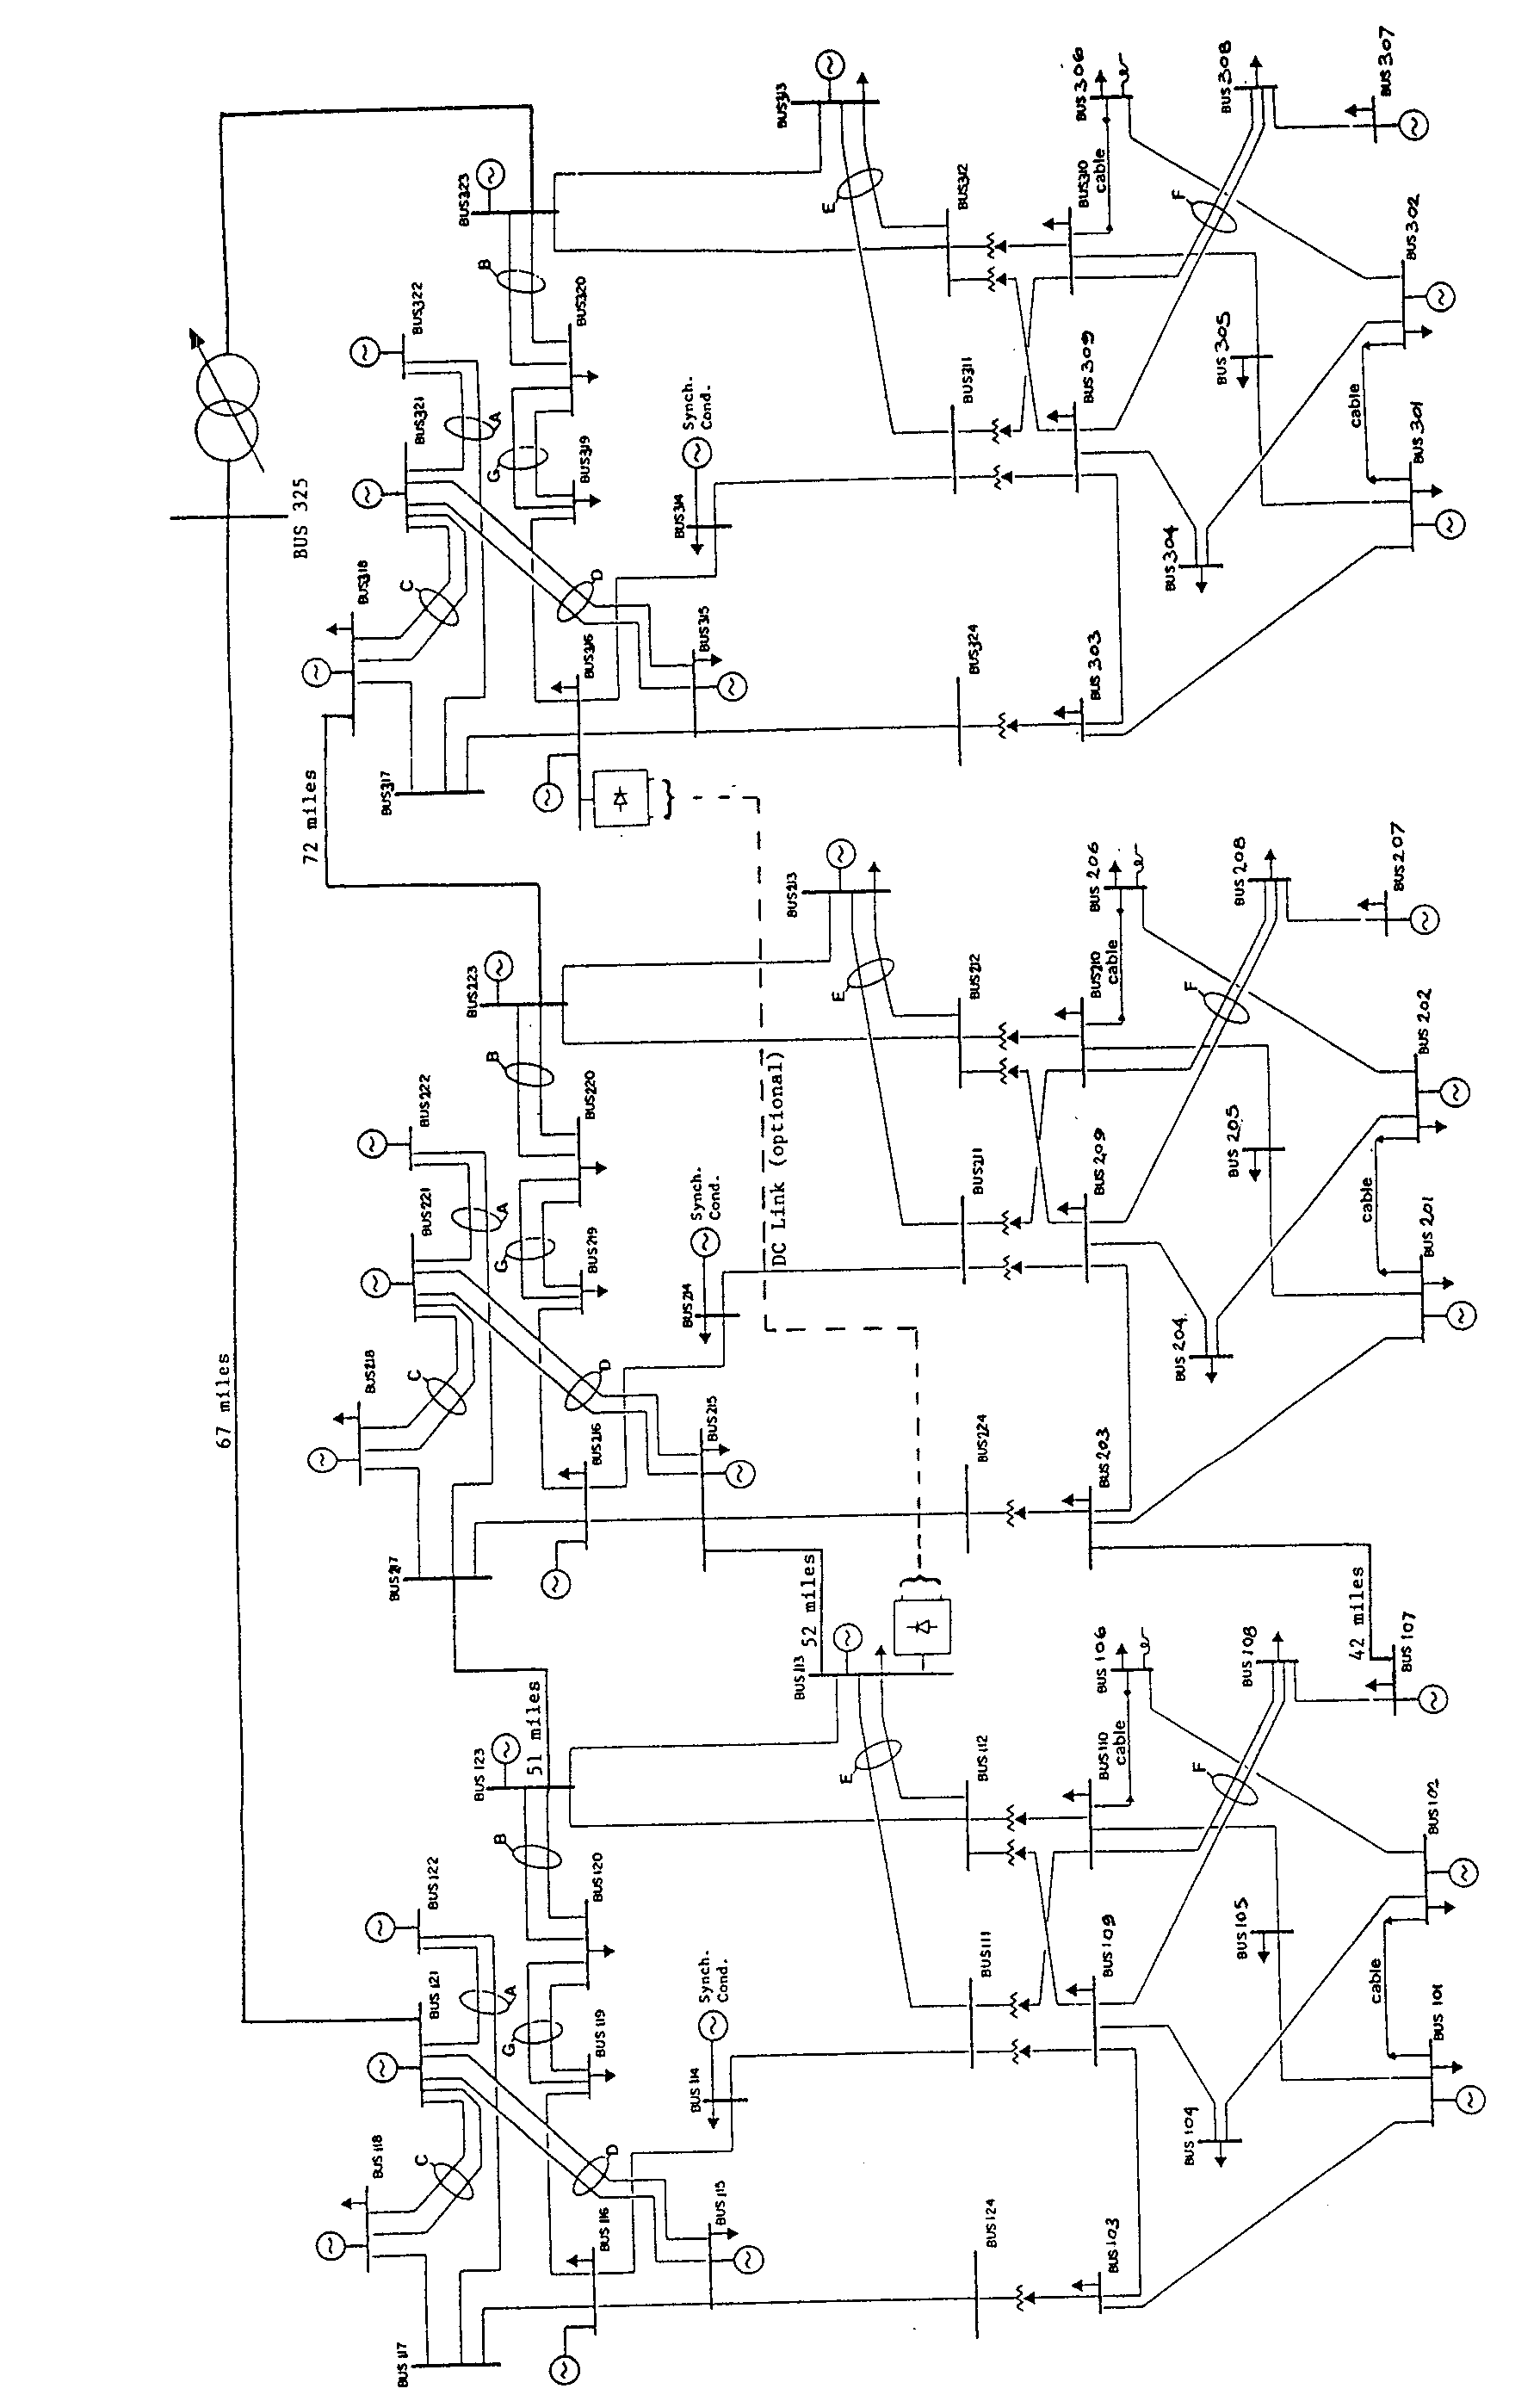
\includegraphics[width=\textwidth,height=\textheight,keepaspectratio]{ieeetopology.png}
  \caption{RTS-96 topology \cite{wongieee}}
  \label{fig:ieeetopology}
\end{figure}

The dataset describes a peak load for each bus. The absolute load in every hour is a percentage the peak load based on 3 components: the week year, the day of week an the hour of the day. The hourly peak changes according to the season and if it is in a weekend or not. For example, the peak load of bus 101 is 108MW. On 01/07 at 12:00 PM the load is:

\begin{multline}
L_{b = 108} =  (L_{yearweek = 27} = 75.5\%) \times (L_{dayofweek = friday} = 94\%) 
\\ \times (L_{hour= 12 PM} = 93\%) \times 108 = 71.28MW
\end{multline}

Figure \ref{fig:totalSystemLoadJuly} displays the total system load throughout the month of July.

\begin{figure}[h!] 
  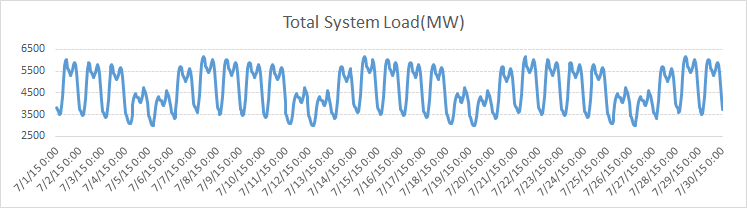
\includegraphics[width=\textwidth,keepaspectratio]{totalSystemLoadJuly.png}
  \caption{System Total Load over the month of July (MW)}
  \label{fig:totalSystemLoadJuly}
\end{figure}

When the models are run under a sub-hourly level,the inter-hour time periods follow the interpolation between the hours with an additional perturbation, following an uniform distribution of $[-Pr,+Pr]\%$, where $Pr$ is a parameter in the range of [0,100]. The objective is to capture the ramping behaviour of NVERs on a sub hourly level. Figure \ref{fig:perturbationDifference} shows a difference between load curve on a 60 minute and 15 minute planning level. 

\begin{figure}[h!] 
  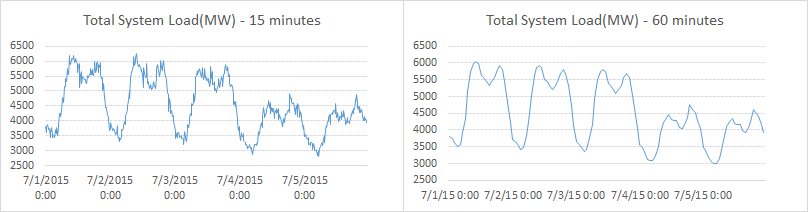
\includegraphics[width=\textwidth,keepaspectratio]{perturbationDifference.png}
  \caption{System Load for 5 days in July under 60 and 15 minutes level}
  \label{fig:perturbationDifference}
\end{figure}

The original RTS-96 system has 87 generators distributed across the test field, with the following generator type distribution:

\begin{itemize}
\item 27 coal/steam generators
\item 18 hydro generators
\item 24 oil/steam generators
\item 15 nuclear generators
\item 3 sync generators (not considered for this study)
\end{itemize}

The total peak load is 8550MW while the total generation capacity is 9975MW. This project assumes the following regarding the data:

\begin{itemize}
\item All the buses follow the same behaviour. Therefore they have positive correlation.
\item The load profile is the same for every year.
\item The peak load is constant and deterministic. No stochastic factor is considered in this study.
\end{itemize}


\subsection{Renewable Generators Data}

Although RTS-96 has most of necessary data for this project, it does not contain any information of renewable generation. Therefore we found necessary to integrate wind and solar data in the field to build realistic results when evaluating the impact of VER's in the proposed models. The wind and solar profiles states the generation capacity for these renewable resources thorough one year, and it is based on historical availability from the last 5 years in Texas.  The data taken was from the Electric Reliability Council of Texas - ERCOT. The geographic renewable potential in Texas were considered for each bus in the system, both for solar and wind generators.

\subsubsection{Wind Profile}


Figure \ref{fig:texasWindProfile} shows the Texas Annual Average Wind speed and the relative geographic positions of RTS-96 buses \cite{wongieee}. The flat northern border is know as the "panhandle" because the state of Oklahoma, in north of Texas, is shaped like a pan. The handle of this pan is where there's most of wind potential in state. In result, most of the new generators are being installed in northwest \cite{texasWindProfile}.

\begin{figure}[h!] 
  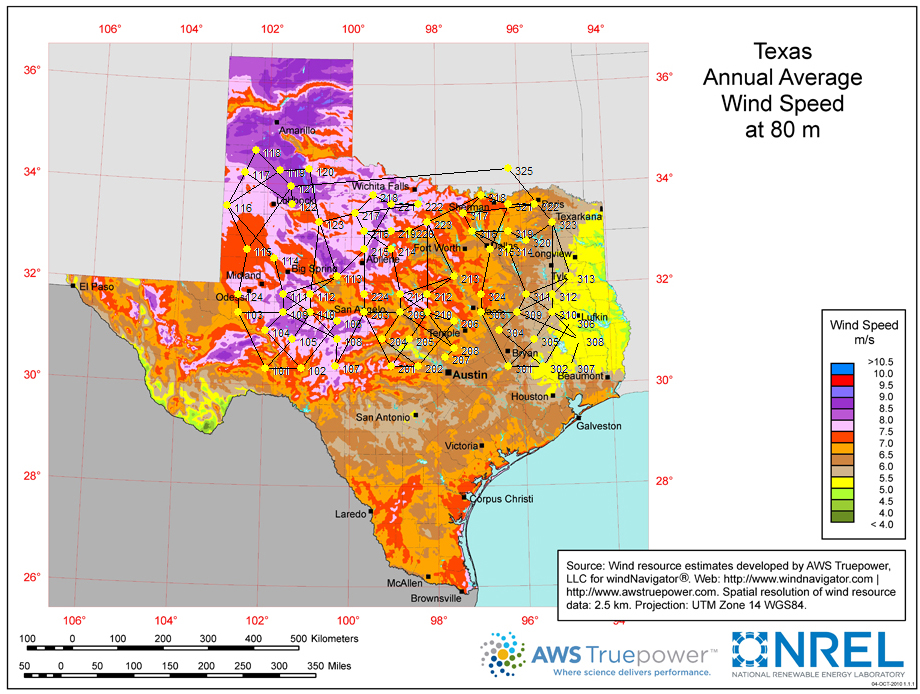
\includegraphics[width=\textwidth,keepaspectratio]{texasWindProfileWithBuses.png}
  \caption{Wind Potential for Texas with RTS-96 Bus Locations. Adapted from \cite{texasWindProfile} }
  \label{fig:texasWindProfile}
\end{figure}


To build the wind potential, each bus were associated to a Texas city or region along with the average historical wind generation for the past 5 years. The studied data is freely shared by ERCOT \cite{ercotGenerationWind}. Therefore each location has a wind potential on an hourly level throughout an entire year. In sub-hourly levels the availability follows the interpolation between the hours followed by an uniform perturbation, using the same logic as load. That said, the real generation for any wind generator is a factor of the percentage of the nameplate capacity followed by the profile where it is located. Figure \ref{fig:windProfileBus122January} shows the wind profile for the bus 122 within the month of January.

\begin{figure}[h!] 
  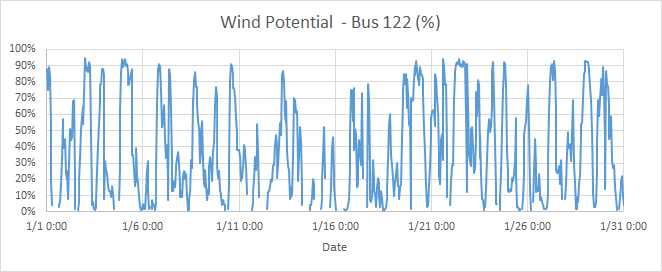
\includegraphics[width=\textwidth,keepaspectratio]{windPotentialBus122.png}
  \caption{Wind Profile for Bus 122 in January}
  \label{fig:windProfileBus122January}
\end{figure}

\subsubsection{Solar Profile}

Figure \ref{fig:texasSolarProfile} displays the NREL's solar incidence report in the state of Texas and the relative geographic positions of RTS-96 buses. 

\begin{figure}[h!] 
	\begin{center}
		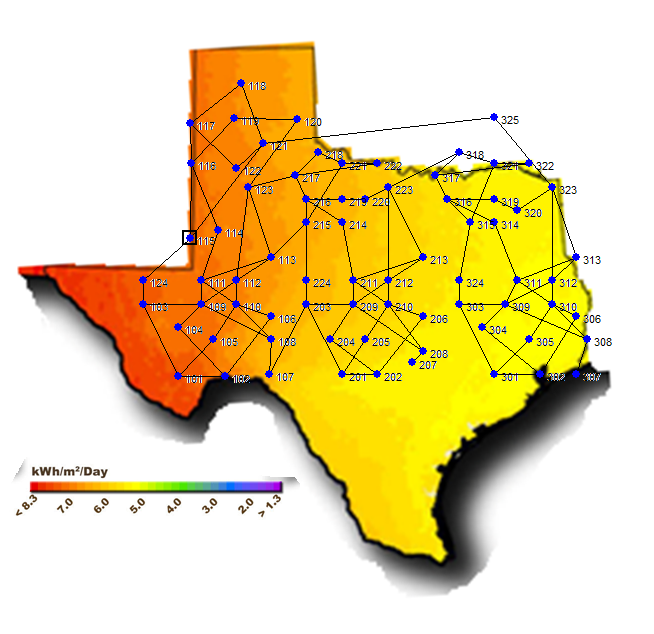
\includegraphics[width=0.6\textwidth,keepaspectratio]{texasSolarProfileWithBuses.png}
	  	\caption{Solar Potential for Texas with RTS-96 Bus Locations. Adapted from \cite{texasSolarProfile} }	  				        \label{fig:texasSolarProfile}
	\end{center}
\end{figure}


It is important to notice that the highest incidence profile in state is located in west of Texas, followed by northeast and center. The solar profile construction followed the same logic developed in the wind case. However, only buses located in the mentioned area had their profiles built. As an example, the solar profile for bus 112 (in far northeast of Texas) on January is shown in figure \ref{fig:solarProfileBus112January}.

\begin{figure}[h!] 
	\begin{center}
		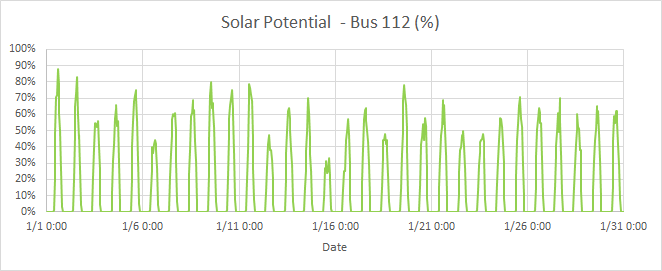
\includegraphics[width=0.8\textwidth,keepaspectratio]{solarPotentialBus112.png}
	  	\caption{Solar Profile for Bus 112 in January }
     	\label{fig:solarProfileBus112January}
	\end{center}
\end{figure}


\subsection{Costs and Assumptions}


\subsection{Scenario Description}

This project studies 3 different generators scenarios under the same demand profile from RTS-96 data. The distribution is adapted from \citeauthor{shavel}, that describes the technical and economical potentials of exploring natural gas and VERs in the state of Texas \cite{shavel}. 

\subsubsection{Scenario 1: Reference}

This scenario captures the existing ERTOC capacity mix. 88\% of generation comes from non-renewable energy sources. The remaining capacity is filled by wind generators, located in the buses that has the Texas Northwest's wind potential (Buses 111-124).

\subsubsection{Scenario 2: Stronger Federal Carbon Rule}

Scenario 2 is build based on column "2032 Total" of table IV-10 in \cite{shavel}. This scenario is described as follows:

\begin{quotation}
"Our scenario with a strong federal carbon rule requires existing coal plants to capture and sequester 90\% of their CO2 output.(...)
As one would expect, this case shows that most of the ERCOT coal plant fleet retires in 2025, the year we assume the carbon rule goes into effect. At this point, 16 GW of coal capacity providing more than 30\% of all ERCOT energy rapidly shifts to gas and renewable supply sources: 6 GW of new CC capacity and 3 GW of new wind capacity. In the next several years, another 3 GW of CC capacity is added, along with another 19 GW of wind. Solar becomes rapidly cost-effective in this scenario and quickly rises to over 8 GW installed by 2029. For the remainder of the scenario horizon, all additional load growth is met by solar and wind additions.”
\end{quotation}

In essence, 44\% of the generation is provided by natural gases, followed by 42\% of NVERs and 14\% of other sources. Most of the wind generators are located at buses 111-124, with some in 211-224. Solar generators are at buses 101-110.


\subsubsection{Scenario 3: "Almost Green World"}

This scenario is an extreme case of Scenario 2. All coal, nuclear and oil/steam generators are not part of the system anymore. The grid runs entirely on wind and solar, with natural gases for ramping, flexibiliy and backup, i.e, to complete the demand whether there is not enough wind and solar to fulfill the load. Wind and solar generators are located throughout the map, following the concentration based on wind and solar profiles from figures \ref{fig:texasSolarProfile} and \ref{fig:texasWindProfile}.

\subsubsection{Scenario 4: "Almost Green World"}

In this scenario all the natural gases are replaced by battery storages. The generation is 100\% provided by wind and solar generators, with nameplate capacity bigger than Scenario 3.

\subsubsection{Generation per Scenario}

The nameplate capacity of base case scenario described by \citeauthor{shavel} is 82,949 MW, where for RTS-96 is close to 10,000 MW. Therefore all absolute generator type capacities were adapted to the new baseline and the rates by type were mantained. The result is in table \ref{table:ScenarioDataDescription}.

\begin{table}[h]
\centering
\begin{tabular}{|lllllll|}
\hline
 & \multicolumn{2}{l}{\textbf{Scenario 1}} & \multicolumn{2}{l}{\textbf{Scenario 2}} & \multicolumn{2}{l|}{\textbf{Scenario 3}} \\ \hline
 & \textbf{MW} & \textbf{\%} & \textbf{MW} & \textbf{\%} & \textbf{MW} & \textbf{\%} \\ \hline
Nuclear & 660 & 6 & 440 & 4 & 0 & 0 \\ \hline
Coal & 2530 & 23 & 220 & 2 & 0 & 0 \\ \hline
Oil/Gas & 1650 & 15 & 880 & 8 & 0 & 0 \\ \hline
NGCC & 4180 & 38 & 4400 & 40 & 2287 & 21 \\ \hline
NGTC & 2090 & 6 & 440 & 4 & 404 & 3 \\ \hline
Wind & 660 & 12 & 3630 & 33 & 7934 & 60 \\ \hline
Solar & 1320 & 0 & 900 & 9 & 2824 & 16 \\ \hline
\textbf{Total} & \textbf{11000} & \textbf{100} & \textbf{11000} & \textbf{100} & \textbf{13452} & \textbf{100} \\ \hline
\end{tabular}
\caption{Total capacity expressed in MW and percentage for each generator type in three scenarios.}
\label{table:ScenarioDataDescription}
\end{table}



\section{Models}

This thesis covers the Economic Dispatch and Unit Commitment models, developed exhaustively in the literature.

\subsection{Indices and Sets}

\begin{tabular}{ll}

$g \in \mc{G} $& Set of generators\\
$b \in \mc{B} $& Set of buses\\
$sd \in \mc{SD} $& Set of storage devices\\
$g \in \mc{G}^{NR} $& Subset of non-renewable generators\\
$g \in \mc{G}^{R} $& Subset of renewable generators \\
$gt \in \mc{GT} $& Set of generator types \\
$u \in \mc{U} $& Set of unit groups \\
$l \in \mc{L} $& Set of transmission lines \\
$rr \in \mc{RR} $& Set of reserve requirements \\
$rp \in \mc{RP} $& Set of reserve products \\
$t \in \mc{T} $& Set of time periods \\
$g \in \mc{G^{b}} $& Set of generators in each bus b \\


\end{tabular}

\subsection{Parameters}

\begin{tabular}{ll}

$D_{b,t} $& Load at bus $b$ in time $t$ \\
$C_{g} $& Generation cost for generator g (\$ / MW) $t$ \\
$S_{g} $& Start-up cost for generator g \\
$R^{up}_{g} $& Ramp up limit for generator g \\
$R^{down}_{g} $& Ramp down limit for generator g \\
$G^{max}_{g} $& Maximum generation capacity for generator g \\
$G^{min}_{g} $& Minimum generation capacity for generator g \\
$T^{min}_{l} $& Minimum transmission of transmission line l \\
$T^{max}_{l} $& Maximum transmission of transmission line l \\
$P^{R}_{g,t} $& Power generation of renewable generator g in time t\\
$U^{up}_{g} $& Minimum uptime of generator g (hours)\\
$U^{down}_{g} $& Minimum downtime of generator g (hours)\\
$ST^{max}_{sd} $& Maximum storage capacity of storage device sd (MW)\\
$ST^{ramp}_{sd} $& Maximum storage capacity of storage device sd (MW)\\

\end{tabular}


Note 1: The generation of renewable resources are not in the decision variables. The developed models only decides the generation for non-renewable resources. Therefore the generation is considered a deterministic parameter, not a variable in the model.

\subsection{Variables}

\begin{tabular}{ll}

$P^{NR}_{g,t} $& Power generation of non-renewable generator g in time t (MW)\\
$T_{i,j,t} $& Power transmitted from bus i to bus j in time t (MW)\\
$T^{loss}_{i,j,t} $& Power loss in transmission from bus i to bus j in time t (MW)\\
$S_{g,t} $& On/off status of generator g at time n\\
$S^{on}_{g,t} $& Start-up status of generator g at time n\\
$S^{off}_{g,t} $& Shut-down status of generator g at time n\\
$V^{-}_{b,t} $& Under generation slack variable at each bus b in time t\\
$V^{+}_{b,t} $& Over generation slack variable at each bus b in time t\\
$ST^{max}_{sd,t} $& Ammount of energy stored in storage device sd in time t\\
$ST^{charge}_{sd,t} $& Ammount of energy charged in device sd in time t\\
$ST^{discharge}_{sd,t} $& Ammount of energy discharged in device sd in time t\\

\end{tabular}

\subsection{Models}

The economic dispatch model satisfies the load and transmission requirements at a minimum cost, following operational requirements such as generation, transmission and ramp limits. In this model, we assume that the commitment decisions has been already made. The main objective function of the studied models is to minimize operational costs over the planning horizon, including fuel, start-up, storage and other variable costs.

The types of constraints that manages the optimal dispatching are:

\begin{itemize}
\item \textbf{Load Constraints:} For each time period, the ammount of power produced and discharge from storage should be equal to the total load and amount charged into a storage. Alternatively, in a node, this equations also considers the inbound and outbound power transmitted.
\item \textbf{Ramping Constraints:}  Each generator has technical limitations that bounds the amount of increase and decrease from one period to next one. This is specially important when there is a considerable load and VERs fluctuations in consecutive periods.
\item \textbf{Generator Limit Constraints:} When turned on, each generator produces a minimum and maximum amount of power, under normal operating conditions.
\item \textbf{Transmission Constraints:} Transfer of power between buses is bounded by the nominal power capacity of the transmission line
\item \textbf{Minimum Reserve Constraints:} These constraints are required to handle the variability and uncertainty of renewable generators. They state that the amount of extra generation must be at least some fraction of generation in that period.
\item \textbf{Storage Constraints:} As well as generators, the charging and discharging rates in storage devices has also technological 


\end{itemize}

\subsubsection{Simple Economic Dispatch Model}

\begin{subequations}\label{model:simple_ED}
\begin{alignat}{4}
min ~~& \sum_{t \in T}\sum_{g \in G^{NR}} P^{NR}_{g,t} C_{g} + \sum_{t \in T}\sum_{b \in B} V^{-}_{b,t} + \sum_{t \in T}\sum_{b \in B} V^{+}_{b,t} \label{eq:ObjectiveFunction} \\
s.t. ~~~& \sum_{t \in T} P^{NR}_{g,t} + \sum_{t \in T} P^{R}_{g,t} + \sum_{t \in T}V^{-}_{b,t} = \sum_{t \in T} D_{b,t}  + \sum_{t \in T}V^{+}_{b,t}  &~& \forall t \in T  \label{eq:loadBalanceConstraint} \\
& P^{NR}_{g,t} - P^{NR}_{g,t - 1} \leq R^{up}_{g} &~& \forall t \in T, g \in \mc{G}^{R}\label{eq:rampUpRateConstraint} \\
& P^{NR}_{g,t -1 } - P^{NR}_{g,t} \leq R^{down}_{g} &~& \forall t \in T, g \in \mc{G}^{R}\label{eq:rampDownRateConstraint} \\
& G^{min}_{g}\leq P^{NR}_{g,t} \leq G^{max}_{g} &~& \forall t \in T, g \in \mc{G}^{R}\label{eq:generationBounds}
\end{alignat} 
\end{subequations}

The constraint \ref{eq:loadBalanceConstraint} states the energy balance in every time. The constraints \ref{eq:rampDownRateConstraint} and \ref{eq:rampUpRateConstraint} states that every generator has to obey the ramp limits. The constraint \ref{eq:generationBounds} states the generation limits for each generator. The use of slack variables $V^{-}_{b,t}$ and $V^{+}_{b,t}$ is necessary to always have feasible solutions, and it is important for scenarios where there is a huge renewable penetrations, when there's an abrupt variation of generation and there is a over or under generation.   

\subsubsection{Economic Dispatch with Transmission Constraints}

In this case, the model has to consider transmission limits and losses, without transmission costs associated. The objective function \ref{eq:ObjectiveFunction} remains the same, and the constraints \ref{eq:rampUpRateConstraint}, \ref{eq:rampDownRateConstraint} and \ref{eq:generationBounds} are als used. The constraint \ref{eq:loadBalanceConstraint} is replaced by  

\begin{subequations}\label{model:edTransmissionConstraints}
\begin{alignat}{4}
&\sum_{g \in G^{b}} P^{NR}_{g,t} + \sum_{g \in G^{b}} P^{R}_{g,t} + \sum_{b^{in} \in B} T_{b^{in},b,t} + V^{-}_{b,t} = D_{b,t}  + V^{+}_{b,t} + \sum_{b^{out} \in B} T_{b,b^{out},t}  &~& \forall b \in B, t \in t \label{eq:transmissionBalanceConstraint} \\
& T^{min}_{l} \leq T_{b^{in},b^{out},t} \leq T^{max}_{l}  &~& \forall b \in B, t \in t \label{eq:transmissionLimits}
\end{alignat} 
\end{subequations}

Constraint \ref{eq:transmissionBalanceConstraint} guarantees that the energy balance is always satisfied for every bus: everything that is generated and received from other buses should be equal to what is loaded and sent throughout the line with the respective losses. If this balance is not satisfied then it is represented in the slack variables. (TODO: put lossed in the equation). The constraint \ref{eq:transmissionLimits} defines the transmission bounds for each line.

\subsubsection{Economic dispatch model with unit commitment constraints}
Unit commitment is the decision of consider the sets of generators that are turned on and off for the planned time horizon. The model includes decision variables to capture ``on'' and ``off'' states for thermal generators in each time period,along with the start-up and shut-down decisions. \citep{palmintier}. The set of constraints are added to the previous model, and the binary nature of the variables makes the problem an MIP, naturally harder to solve computationally \cite{james}. 

\begin{subequations}\label{model:ucConstraints}
\begin{alignat}{4}
& S_{g,t} = S^{on}_{g,t} - S^{off}_{g,t} + S_{g,t}  &~& \forall g \in \mc{G}^{NR} , t \in \mc{T} \label{eq:logconst}\end{alignat} 
\end{subequations}

Constraint \ref{eq:logconst} specifies the logical condition between the binary variables, assuring that a generator can not be on if it was not turned on. The same is valid for turning it off. Constraints \ref{eq:mindownt} and \ref{eq:minupt} forces the generator to follow their minimum downtime and uptime periods when they are turned on or off. 

When there is the decision of turning the generator on or off, ramping and transmitting only makes sense if the generator is on in a certain time period. Therefore these constraints has the corresponding binary variable, as shown in \ref{model:UC_NewConstraints}.

\begin{subequations}\label{model:UC_NewConstraints}
\begin{alignat}{4}
& P^{NR}_{g,t} - P^{NR}_{g,t - 1} \leq R^{up}_{g} S_{g,t} &~& \forall t \in T, g \in \mc{G}^{R}\label{eq:UCrampUpRateConstraint} \\
& P^{NR}_{g,t -1 } - P^{NR}_{g,t} \leq R^{down}_{g} S_{g,t} &~& \forall t \in T, g \in \mc{G}^{R}\label{eq:UCrampDownRateConstraint} \\
& G^{min}_{g} S_{g,t}\leq P^{NR}_{g,t} \leq G^{max}_{g} S_{g,t} &~& \forall t \in T, g \in \mc{G}^{R}\label{eq:UCgenerationBounds}
\end{alignat} 
\end{subequations}
 
It is important to highlight that if a generator is down in previous period so it can reaches the minimum generation level in the period it is on; otherwise it can not exceed the ramping rate <make it better here>

In unit commitment model, each generator must satisfy a minimum period to remain on or off whether there is a state change on a certain period. Down time constraints are  useful to keep maintenance of a generating unit once has been shut down. Uptime constraints are useful to guarantee stability and reduces stress of equipments. 

\begin{subequations}\label{model:ucMinDownUpConstraints}
\begin{alignat}{4}
& \sum_{i = t}^{t + U^{up}_{g} - 1} S_{g,t} \geq S^{on}_{g,i} U^{up}_{g} &~& \forall g \in \mc{G}^{NR}, t \in \mc{T} \label{eq:mindownt} \\
& \sum_{i = t}^{t + U^{down}_{g} - 1} (1 -S_{g,t}) \geq S^{off}_{g,i} U^{down}_{g} &~& \forall g \in \mc{G}^{NR}, t \in \mc{T} \label{eq:minupt}
\end{alignat} 
\end{subequations}

\subsubsection{Economic Dispatch/Unit Commitment with Storage Constraints}

Under a scenario where renewable resources are the major source of energy, storage devices are crucial to address fluctuations and uncertainties in generation, so they are an important key to keep the system stable \cite{dwyer}. When storage devices are available in the system, their operations are ruled by the following constraints:

\begin{subequations}\label{model:storageConstraints}
\begin{alignat}{4}
& ST^{max}_{sd,t} = ST^{max}_{sd,t - 1} + ST^{charge}_{sd,t} - ST^{discharge}_{sd,t}  &~& \forall sd \in SD, t \in t \label{eq:storageLimits} \\
&  -ST^{ramp} \leq (ST^{charge}_{sd,t} - ST^{charge}_{sd,t-1}) + (ST^{discharge}_{sd,t} - ST^{discharge}_{sd,t-1}) \leq ST^{ramp}  &~& \forall sd \in SD, t \in t \label{eq:storageRamping}
\end{alignat} 
\end{subequations}


\section{Implementation}


\subsection{Software Selection}

During the briefing process, it was necessary to choose the software platform that matches our project goals, such that it allows the development, run an analysis the project feasible time. 3 options were considered:

\subsubsection{MATPOWER}

MATPOWER is a powerfull tool designed to solve AC and DC Power Flow (PF) and Optimal Power Flow (PF) problems. It is an add-on to MATLAB, and is mainly used for education and research, with a small use on industry. \cite{zimmerman} Although \citeauthor{zimmerman} states that is is possible to dispatch the generators on a minimal quadratic or linear cost, it has limitations on committing them, i.e., starting up or shutting down on a multi-period environment. MATPOWER is very powerful on a single time period, but it can provide computational challenges for multi-periods on a larger horizon. Therefore we concluded this tool was not appropriate for this project.

\subsubsection{PLEXOS \textregistered }

PLEXOS \textregistered is a commercial tool to power systems planning, widely used in power industry to energy resources planning and analysis. It provides academic license, although the process is long. One of reasons to not use it was the necessity to use commercial nature of the tool, which could lead to challenges in make everything developed in this thesis available to academic community.  

\subsubsection{AIMMS}


AIMMS is a mathematical programming tool designed to solve optimization problems. It is as powerful as other optimization tools like AMPL, GAMS. Some features include \cite{bisschop}:

\begin{itemize}
\item Easy-to-use design of complex parameters
\item Intuitive representation of calendar and time horizons
\item Set of optimization tools to solve LP, QP, NLP and MINLP problems
\item GUI to build end-user interfaces
\item Open Data Base Connectivity (OBDC) and OLE interfaces, allowing data exchange between most common databases, as Oracle, SQL Server, etc.
\end{itemize}

Due to easiness of use, the fact that an academic license provides 100\% of the tool functionality, and the previous experience of the members of this project, AIMMS was chosen as the supporting tool for this work. The software features are described in next section.

\section{Software Features}

This section briefly covers all the screens and features developed in AIMMS for this project.

\subsubsection{Data Import}

The data import section allows the user to import all the data using the AIMMS specific structure for data text exchange. More details on how prepare the data can be found at \cite{bisschop2006aimms}.

\begin{figure}[h] 
	\begin{center}
		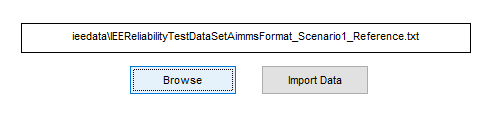
\includegraphics[keepaspectratio]{aimmsScreenImportPage.png}
	  	\caption{Data Import page in AIMMS}
     	\label{fig:aimmsScreenImportPage}
	\end{center}
\end{figure}

\subsubsection{Data Settings}

After the data has been imported, the user has the chance to add/edit and view some data on an intuitive way. In \textit{Network Page}, it is possible to see the location of buses (in yellow), as well as locations of generators per type. The user can change the list to see whatever type he wants. In \textit{Data Buses Page}, it is possible to edit the peak load of each bus in the system. The \textit{Costs Page} has the start-up and variable cost for each generator type and unit group. In \textit{General Data Page} the user can add, edit and remove the main components of the system, i.e., buses, generators and unit groups, as well as changing general configurations, such as horizon dates, granularity and perturbation level for load and wind profiles under a sub-hourly level. 

It is possible also to see the total load over time. In \textit{Generators Specification Page} it is possible to configure the main parameters that defines a generator, such as its type, unit group and bus where it is located. In \textit{Wind and Solar Availability Page} it is possible to view the Wind and Solar profile for the selected bus in the node, as well as locations that have either solar or wind profile mapped (marked with the blue ball). Lastly, the \textit{Summary Page} summarizes the total generation capacity and load, as well as total number of generators and its capacity per generator type.

\begin{figure}[h] 
	\begin{center}
		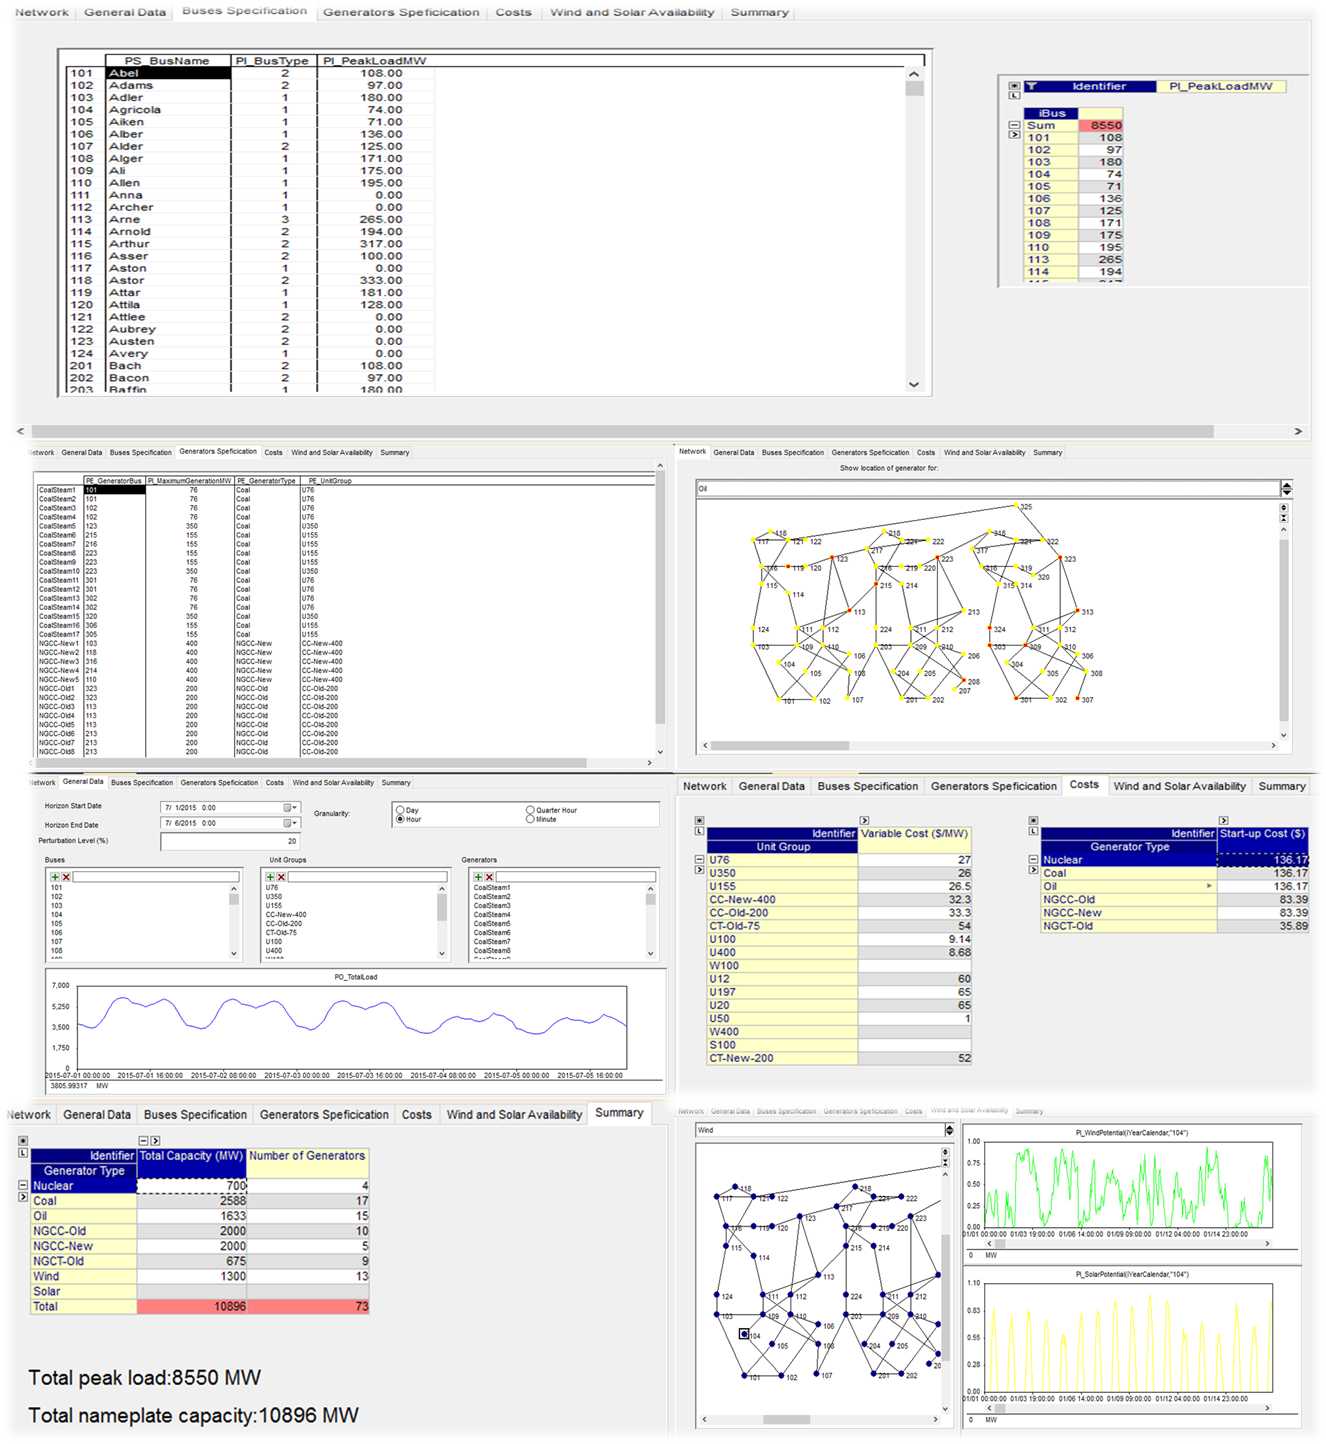
\includegraphics[width=\textwidth,height=\textheight,keepaspectratio]{aimmsDataPages.png}
	  	\caption{Data Section Pages}
     	\label{fig:dataSectionPages}
	\end{center}
\end{figure}


\subsubsection{Optimization and Results}

The optimization section contains all the required settings to run the optimization, as well as the tables and graphs to analyse the results on an intuitive way. 

The user has the option either to solve the Economic Dispatch or Unit Commitment problems, with or without the following features:

\begin{itemize}
\item Ramping Constraints
\item Transmission Constraints
\item Reserve Constraints
\item Slack Variables
\item Transmission Losses (if "Transmission Constraints" is chosen)
\end{itemize}

In \textit{Demand, Load and Transmission}, it is possible to see, for every bus in every time period, the load, generation and transmission flows in and out. It also is possible to see this same flow on a graphic way in \textit{Transmission Map} section, for each time time period, as well as the location of VERs(in green) and active(red) and inactive(gray) NVERs. The \textit{Average Load Distribution} contains the graph displaying the average load for each generator type within a day, while in \textit{Load Distribution Page} it is possible to see the generation distribution per time period, as well as the total load, being useful to identify over and under generation. The \textbf{Power Output Result} details the generation by each generator, in a table. Finally, the \textit{Location Marginal Prices} page contains the Shadow Prices per time for each location, and it is useful to identify potential investments or bottlenecks.

The \textit{Average Ramping} page is useful to compare the ramping behaviour of the generator sources, expressed as:

\begin{equation}
    AverageRamping_{gt \in \mc{GT}} = \overline{\dfrac{P^{NR}_{g,t} - P^{NR}_{g,t-1}}{G^{max}_{g}}}
\end{equation}

In other words, it expresses the average ramping grouped by each generator type , normalized by its maximum capacity. It avoids the misunderstanding of high-capacity generators being ramped more than the lower ones.

\begin{figure}[h] 
	\begin{center}
		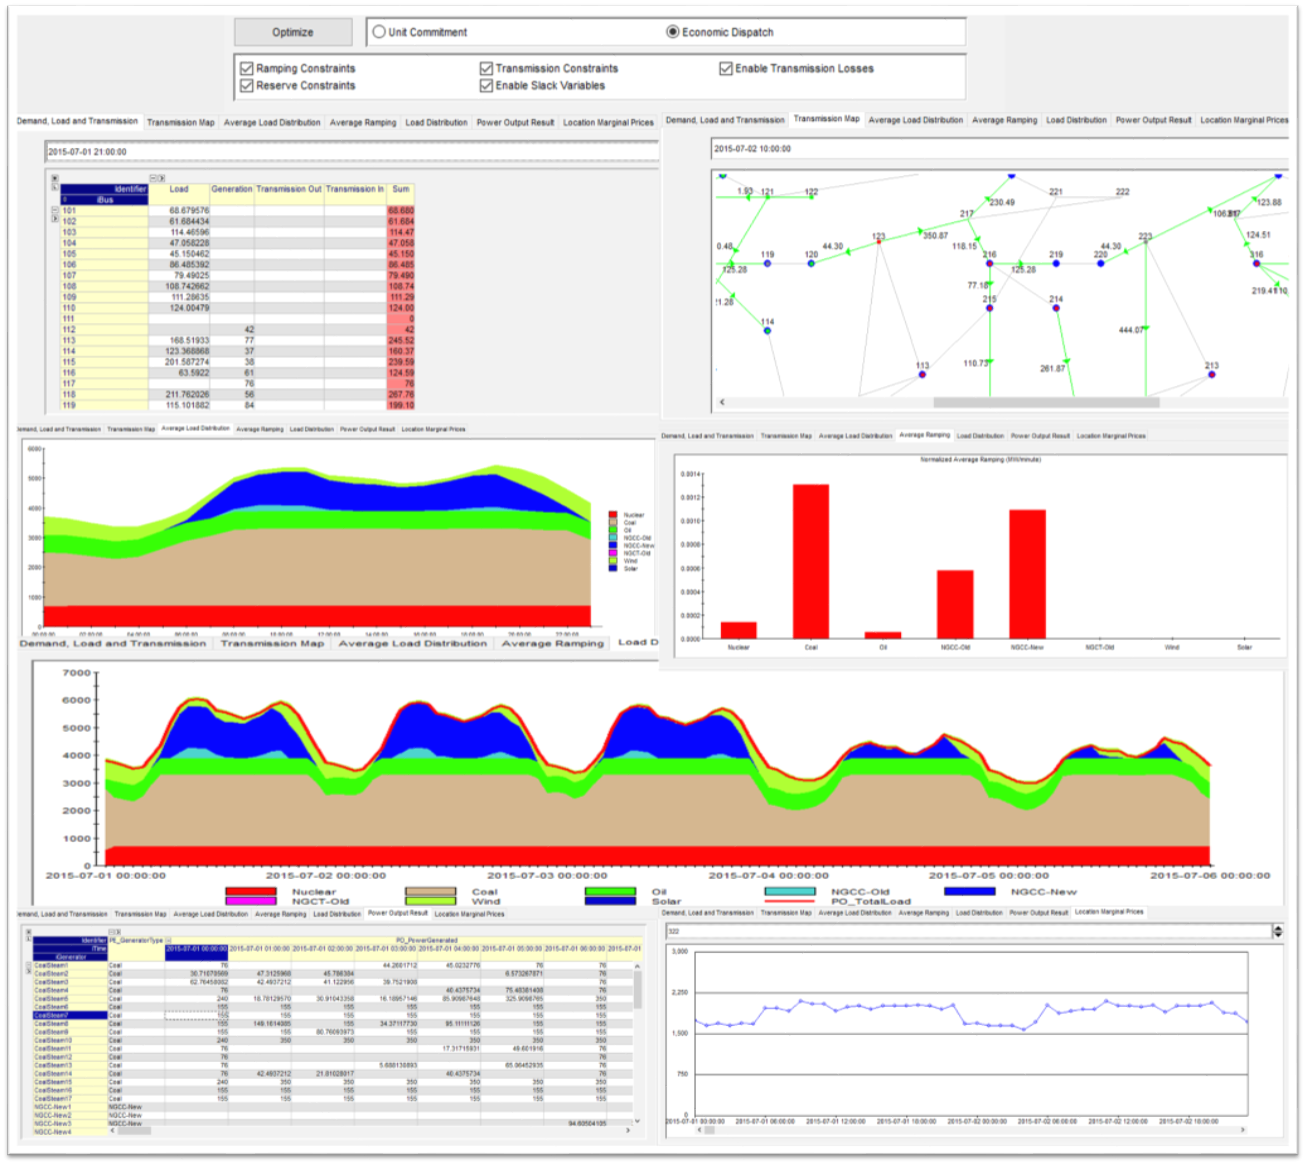
\includegraphics[width=\textwidth,height=\textheight,keepaspectratio]{aimmsOptimizationSectionPages.png}
	  	\caption{Optimization Section Pages}
     	\label{fig:optimizationSectionPages}
	\end{center}
\end{figure}


\addcontentsline{toc}{chapter}{Analysis}
\chapter{Analysis}

In the analysis make all the scenario runs, describe all the scenarios test, put a table with all the possibilities, and categorize them by model and describe then. Then, make an analysis by ramping, over and under generation, as well as results. Put graphs, tables, everything that supports your points of view.

The analysis has the goal to evaluate the impact of the following components in UC and ED models:

\begin{itemize}
\item Time granularity: 1 hour, 15 minutes and 5 minutes
\item Transmission: with or without transmission
\item Level of VERs: Scenarios 1, 2 and 3
\end{itemize}

With all possible combinations of these factors, there are 36 data sets to analyse. These are defined as "test cases", as described in table Create the Table. The following parameters are object of analysis:

\begin{itemize}
\item Power Output per generation type over time
\item Under and Over Generation over time per bus
\item Running time per test case
\item Ramping distribution for NVERs per generator type
\end{itemize}

\subsection{Power Output per Generation Type}

Figures \ref{fig:powerOutputScenario1}, \ref{fig:powerOutputScenario2} and \ref{fig:powerOutputScenario3} has the power production for each generator type in a combination of model type (UC or ED), granularity (60, 15 and 5 minutes) and transmission constraints on and off. Each figure represents the result for each scenario described in the Data Section. All instances represent the same time period of one week of July, with the same load profile. The generator type colors are described at the bottom of the page, and to make the curve more analysis friendly all the x-axis were removed. There are some interesting analysis, which will be described by Scenario.

\subsubsection{Scenario 1}

- When there is no transmission constraints, there was no significant difference of generation distribution between time granularities on the Economic Dispatch version, except for the ramping behaviour of non-renewable resources. It is expected to ramping more due to the variability under a sub-hourly level. 
- The generation profile is the same for nuclear, coal and oil sources for the economic dispatch model. When the model is solved with transmission constraints, only NGCC-New generators can not handle the demand under the peak, so they need to be complemented by NGCC-Old ones. The reason for that is the transmission limit on power transmission, wich does not allow NGCC-New generators to fill all the left demand at peak, letting NGCC-New generators supply it.
- As for Unit Commitment with Transmission Constraints on a 60-minute level, the NGC-Old generators were turned on during the running process, and remained until the end of the horizon, which reduced the generation of base generators during low demand,specially Nuclear types.
- When UC decisions were made on sub-hourly levels, the generation distribution profile differed from the other configurations significantly, which lead to a further investigation. On a 15 minute-level the optimizer decided to turn on most of natural gas generators (NGCC-New, NGCC-Old, NGCT-New) and use NGCT-Old generators to fulfil peak demands, cheaper start-up option than Oil and Coal, and keep few oil generators running at a minimal level. However for the first three days the total demand was not fulfilled during peak load. 

The generatio

For a 5 minute level the MIP was not able to do the resource planning,  allowing the demand to be unmet, for both transmission cases. We decided to investigate this result better, with different levels of normal perturbation. 





\subsubsection{Scenario 2}

\subsubsection{Scenario 3}

\begin{figure} 
  \centering
  
	  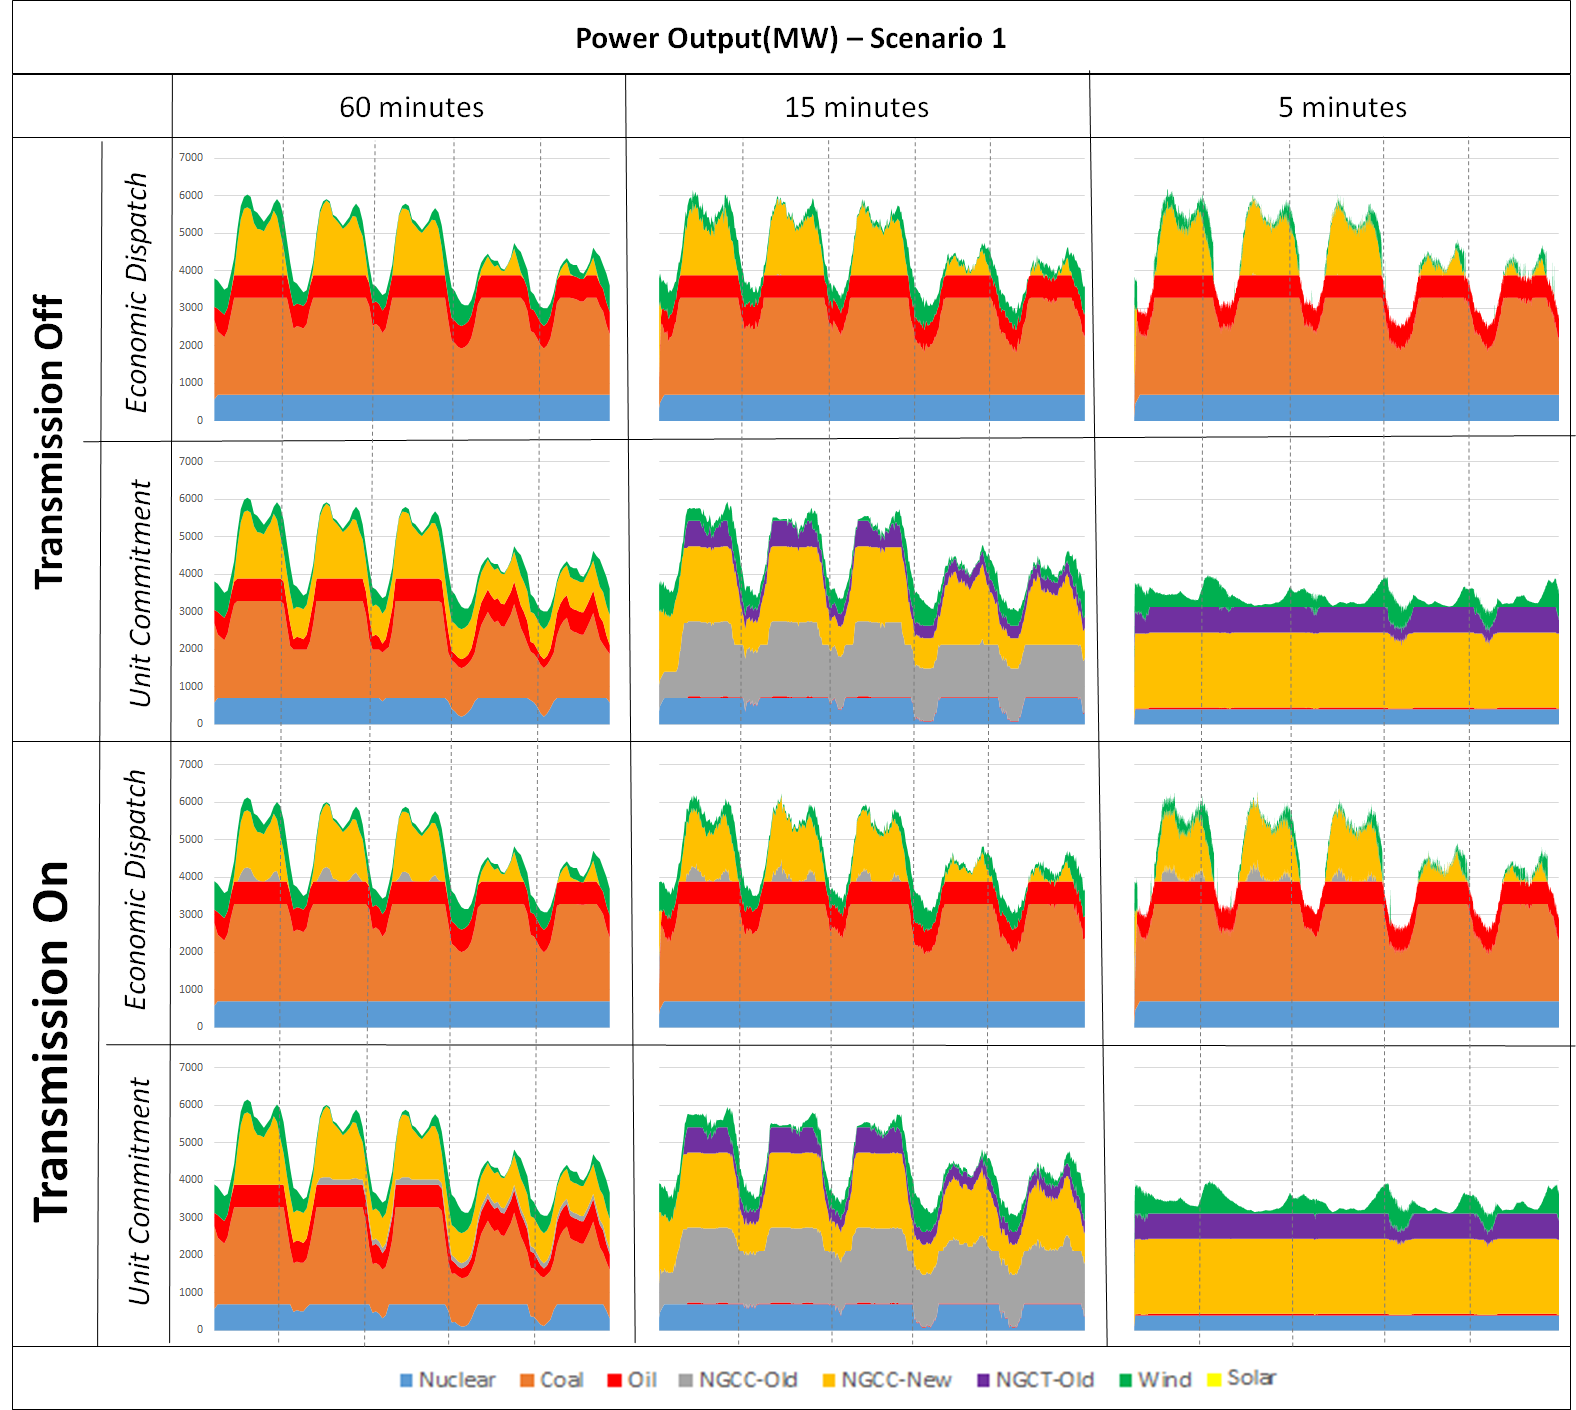
\includegraphics[width=\textwidth,height=\textheight,keepaspectratio]{PowerOutputScenario1.png}
  
  \caption{Power Output for Scenario 1.}
  \label{fig:powerOutputScenario1}
\end{figure}

\begin{figure} 
  \centering
  
	  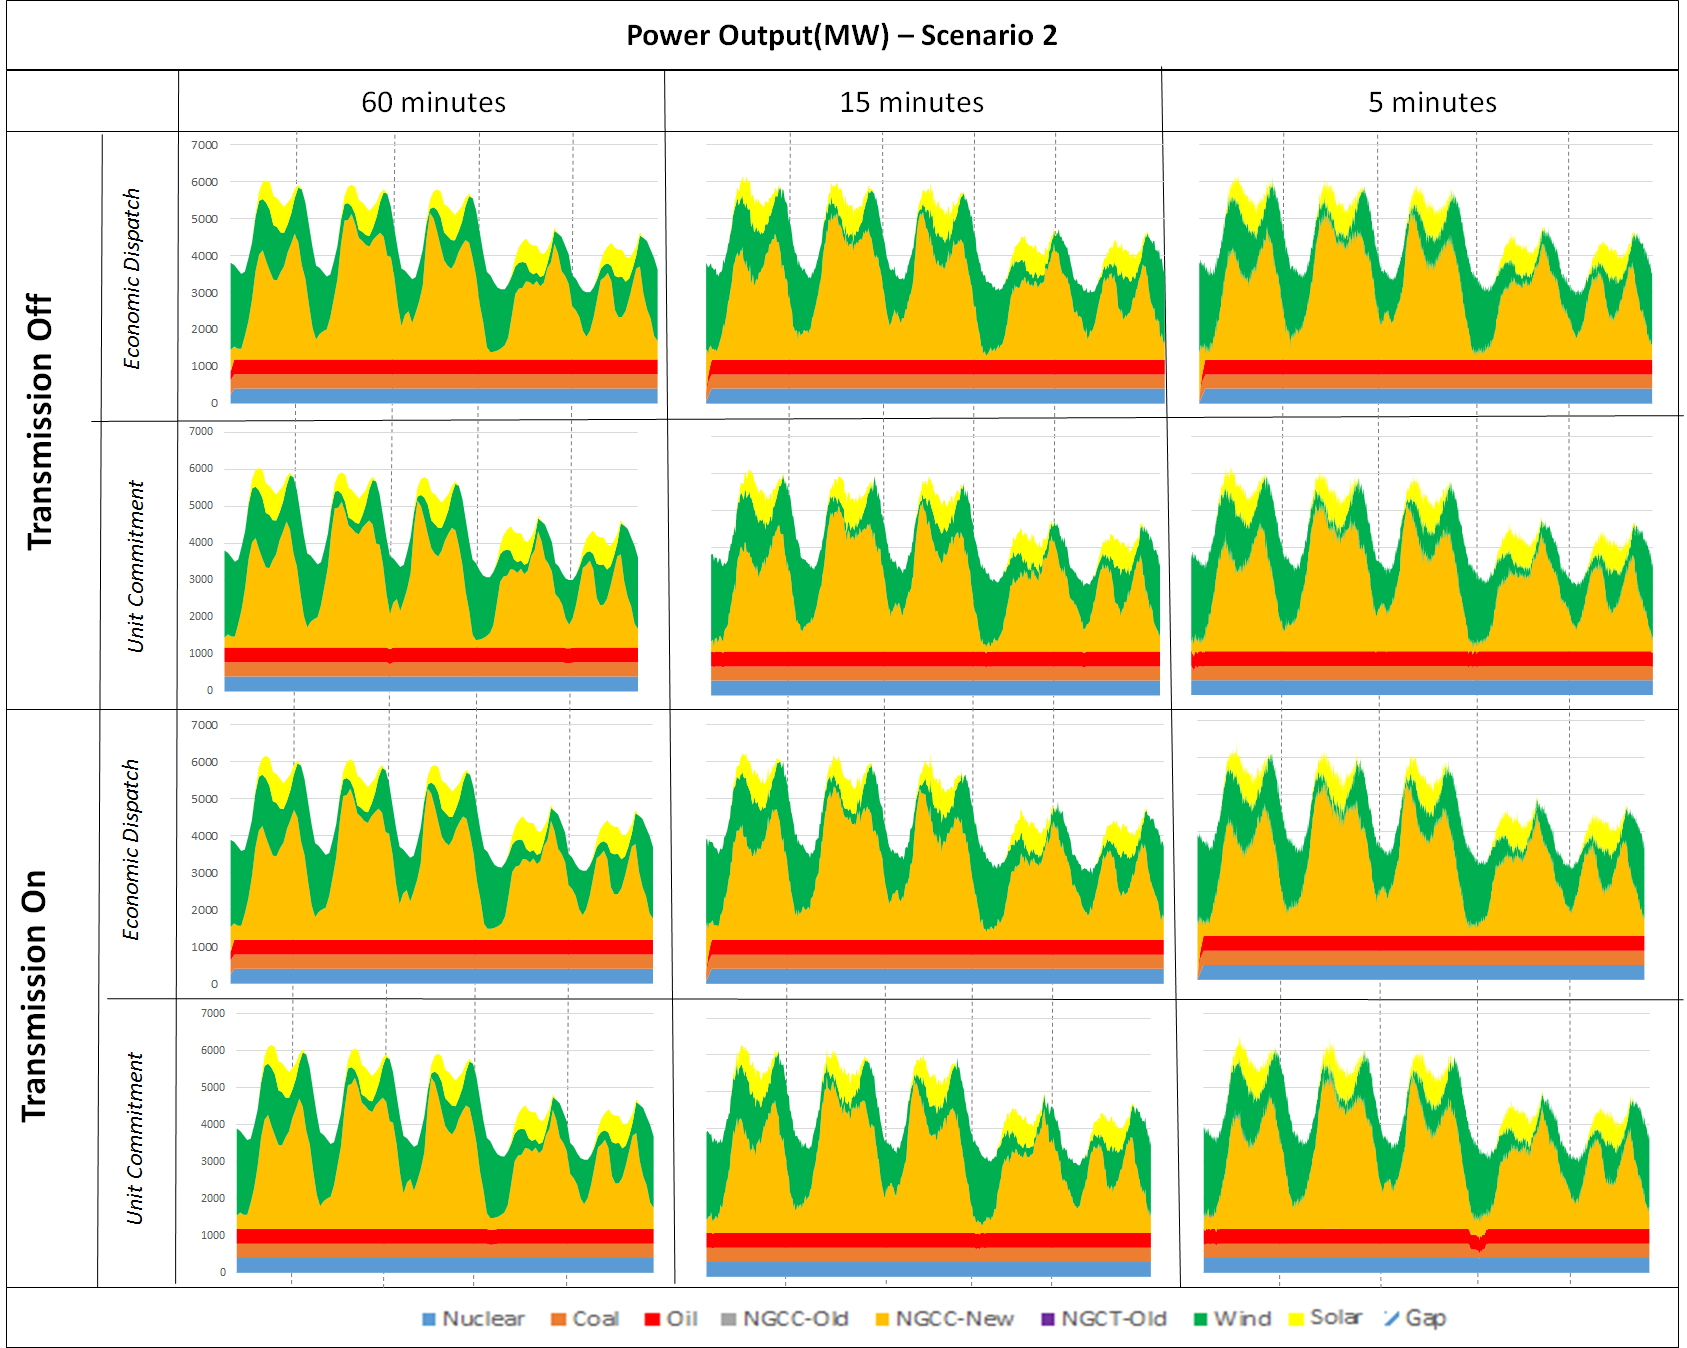
\includegraphics[width=\textwidth,height=\textheight,keepaspectratio]{PowerOutputScenario2.png}
  
  \caption{Power Output for Scenario 2.}
  \label{fig:powerOutputScenario2}
\end{figure}

\begin{figure} 
  \centering
  
	  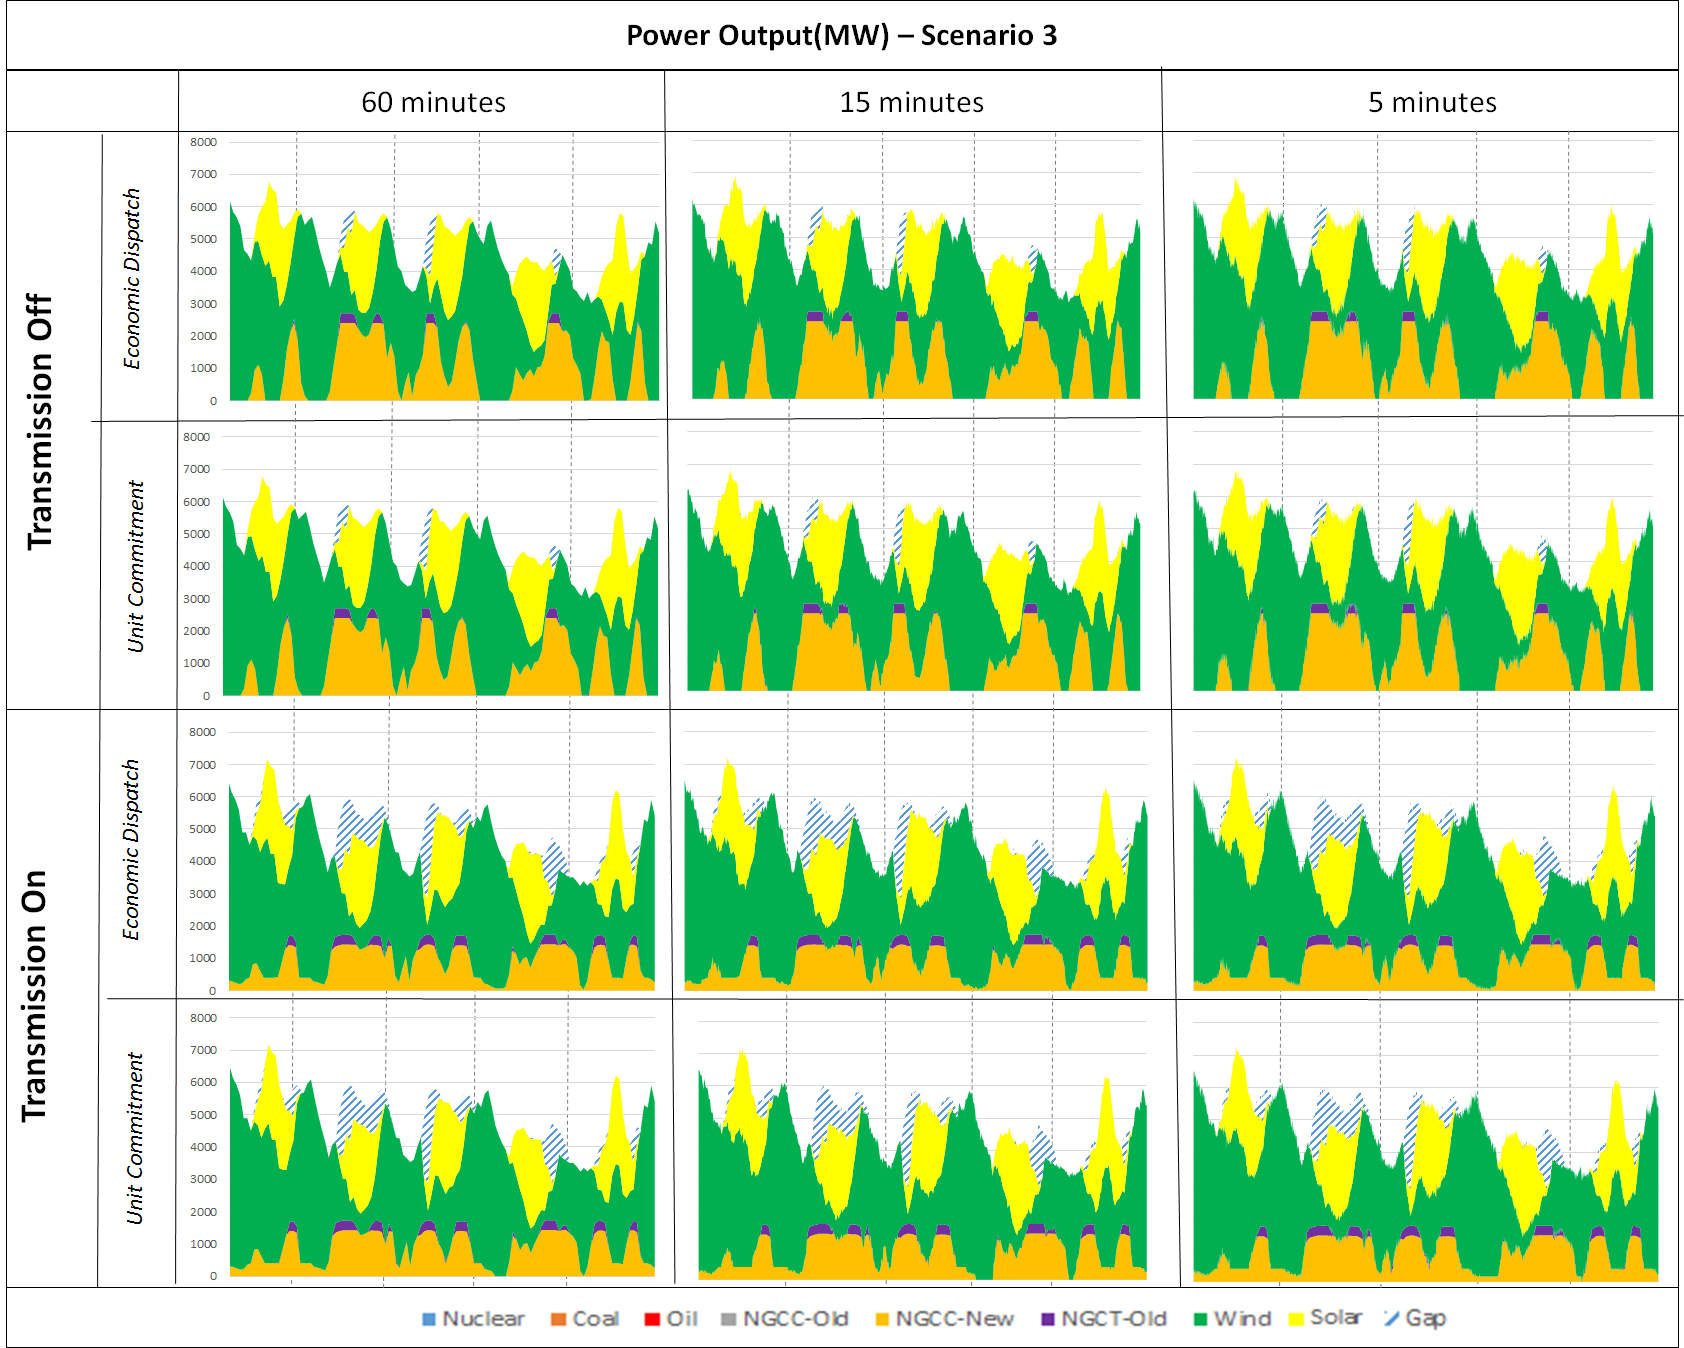
\includegraphics[width=\textwidth,height=\textheight,keepaspectratio]{PowerOutputScenario3.png}
  
  \caption{Power Output for Scenario 3.}
  \label{fig:powerOutputScenario3}
\end{figure}



\addcontentsline{toc}{chapter}{Conclusion}
\chapter{Conclusion}

\appendix
%\chapter{Power Systems Operation Background}

%\chapter{Data and Analysis}

\bibliographystyle{plainnat}
\nocite{*}
\bibliography{biblio}
%\addcontentsline{toc}{chapter}{Vita}
\chapter*{Vita}
\addcontentsline{toc}{chapter}{Vita}

Daniel Xavier Wolbert was born in 7 July of 1987 in Brazil, son of Cleber Wolbert and Mirian Xavier. He attended Universidade Federal de Minas Gerais in Brazil, graduating in December of 2010 in B.S. of Control and Automation Engineering. From 2010 to 2013, he acted as business and systems consultant at Accenture. He attended Lehigh University to obtain his M.S. in Industrial and Systems Engineering in May 2016. He was awarded as the "ISE Master's Student of The Year Award" in 2016.
\end{document}

